\chapter{ทฤษฎีที่เกี่ยวข้อง}
บทนี้จะเป็นรายละเอียดเกี่ยวกับทฤษฎีและงานวิจัยที่เกี่ยวของกับการพัฒนาโปรแกรมในครั้งนี้ โดยที่แต่ละหัวข้อจะมีความสัมพันธ์กันเป็นลำดับ โดยหัวข้อที่หนึ่งจะแนะนำความรู้เรื่อง Python เพื่อให้เข้าใจพื้นฐานเบื้องต้นเกี่ยวกับที่มาของโครงงาน หัวข้อที่สองที่สามจะช่วยเตรียมให้ผู้อ่านเข้าใจเทคโนโลยที่ใช้ในการออกแบบและพัฒนา ส่วน ...

\section{ความรู้พื้นฐานเกี่ยวกับ Python}
	Python  คือ ภาษาเขียนโปรแกรมระดับสูงที่ใช้กันอย่างกว้างขวางในการเขียนโปรแกรมสำหรับวัตถุประสงค์ทั่วไป ภาษา Python นั้นเป็นภาษาแบบ Interprete ที่ถูกออกแบบให้โค้ดอ่านได้ง่ายขึ้น และโครงสร้างของภาษานั้นจะทำให้โปรแกรมเมอร์สามารถเข้าใจแนวคิดการเขียนโค้ด โดยใช้บรรทัดที่น้อยลงกว่าภาษาอย่าง C++ และ Java ซึ่งภาษานั้นถูกกำหนดให้มีโครงสร้างที่ตั้งใจให้การเขียนโค้ดเข้าใจง่าย ทั้งในโปรแกรมเล็กไปจนถึงโปรแกรมขนาดใหญ่ คุณลักษณะเด่นของภาษา Python 
    \begin{enumerate}
    	\item สนับสนุนแนวแบบคิดออปเจกต์โอเรียนเทด หรือ OOP (Object Oriented Programming)
    	\item เป็น Open Source
    	\item โค้ดที่เขียนด้วย Python สามารถนำไปรันบนระบบปฏิบัติการได้หลากหลาย
    	\item สามารถประมาลผมทางด้านวิยาศาสตร์ และวิศวกรรมศาสตร์ได้อย่างมีประสิทธิภาพ
    	\item มีฟังก์ชันสนับสนุนฐานข้อมูล เช่น MySQL, Sybase, Oracle , Informix, ODBC และอื่นๆ
    	\item มี Library สนับสนุนด้านการสร้างภาพกราฟฟิก ตลอดจนบันถึกไฟล์ในรูปแบบต่างๆ ได้อย่างสะดวกและมีประสิทธิภาพ
    	\item มี Library สนับสนุนด้านปัญญาประดิษฐ์
    \end{enumerate}
    

	\section{ความรู้พื้นฐาน Django Framework}
	Django Framework  คือ ชุดเครื่องมือ Framework สำหรับ การพัฒนาเว็บไซต์ด้วยภาษา Python ซึ่งความเป็นจริงแล้วทุกวันนี้มี Framework สำหรับการเขียนเว็บไซต์ด้วยภาษา Python ค่อนข้างเยอะ ซึ่ง Django Framework เป็นหนึ่งใน Framework สำหรับการพัฒนาเว็บไซต์ และทำเว็บไซต์ด้วยภาษา Python ด้วยเช่นกัน โดยปัจจุบันภาษา Python นั้นค่อนข้างได้รับความนิยมเพิ่มมากขึ้น  Django Framework \cite{django} มีคุณสมบัติดังนี้
	
	\begin{enumerate}
		\item Object-relational mapper คือ การกำหนด Data Model ในภาษา Python เพื่อการทำงานด้านข้อมูล และสนับสนุน Dynamic database-access API
		\item Automatic admin interface คือ ส่วนของการสร้าง Interface อัตโนมัติสำหรับการ add, edit , delete และ search ด้วย Django Framework
		\item  Elegant URL design คือ การทำให้ URL มีความสวยงาม สั้น กระชับ และสื่อความหมายของหน้านั้น ๆ ได้อย่างชัดเจน เหมาะสมกับการทำ SEO ในปัจจุบัน
		\item Template system คือ Django นั้นมีการออกแบบ Template Language เพื่อการเขียนแยกส่วนระหว่าง Design และ Business Logic
		\item Cache system คือ ส่วนของการบันทึก หรือจัดการข้อมูลที่มีการดาวน์โหลดไปแล้ว เพื่อเพิ่มประสิทธิภาพการทำงานของเว็บไซต์ด้านความเร็ว และด้านอื่น ๆ
		\item Internationalization คือ Django สนับสนุน Application ที่มีความหลากหลายด้านภาษาในการแสดงผล
	\end{enumerate}
	รูปแบบ MVC ของ Django   เรียกอีกอย่างว่า MTV คือ Model Template View ดังรูปที่  \ref{Fig:Django}
	
	\begin{figure}[H]
		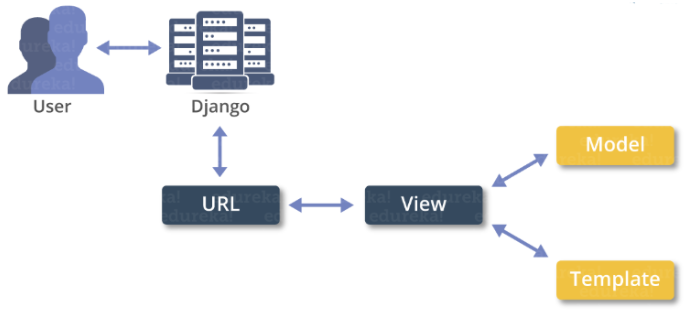
\includegraphics[width=\columnwidth]{Figures/insect2/django}
		\caption{รูปแบบ MVC ของ Django}{ที่มา: https://www.edureka.co/blog/django-tutorial/}
		\label{Fig:Django} 
	\end{figure}
	
	
	
    \end{itemize}
	
\section{ความรู้พื้นฐานเกี่ยวกับ Bootstrap}
Bootstrap  คือ Front-end Framework ที่ช่วยให้สามารถสร้างเว็บแอปพลิเคชันได้อย่างสวยงาม ตัว Bootstrap มีทั้ง CSS Component และ JavaScript Plugin ให้เรียกใช้งานได้ และยังถูกออกแบบมาให้รองรับการทำงานแบบ Responsive Web ซึ่งทำให้ การพัฒนาเว็บแค่ครั้งเดียวสามารถนำไปใช้งานบนเบราเซอร์ใน มือถือ แท็บเล็ต และคอมพิวเตอร์ ได้ และผู้พัฒนาไม่ต้องมีความรู้ด้าน CSS มาก  สามารถสร้างเว็บที่สวยงามได้เช่นกัน

\section{ความรู้พื้นฐานเกี่ยวกับ OpenCV(OpenSourceComputerVision)}
OpenCV  เป็น Library ที่รวบรวมฟังก์ชันสำหรับการประมวลผลภาพและคอมพิวเตอร์วิทัศนศาสตร์ ไว้เป็นจำนวนมากอยู่ภายใต้ใบอนุญาต BSD ซึ่งสามารถใช้ได้ฟรีทั้งทางด้าน การศึกษาและทางการค้า เนื่องจากนี้ยังมีการประยุกต์ใช้งาน OpenCV  ในแบบต่างๆ ได้แก่ ระบบตรวจจับใบหน้า (Face Detection) การจดจำใบหน้า (Face Recognition) การติดตามวัถตุ (Object Tracking) การเรียนรู้ของเครื่อง (Machine Learning) เป็นต้น

\subsection{การประมวลผลภาพ (Image Processing)}
การประมวลผลภาพคือการนำรูปที่มีอยู่แล้ว หรือรูปที่รับเข้ามาจากอุปกรณ์ต่างๆ หรือรูป ที่มีอยู่มาประมวลผลเพื่อหาลักษณะเด่นบางประการของรูปที่มีอยู่ หรืออาจจะเป็นการตีความ หมายของภาพรวมถึงการปรับคุณลักษณะของภาพให้เป็นไปตามต้องการโดยใช้กระบวนการทาง คณิตศาสตร์ 
การประมวลผลภาพแนวคิดทางคณิตศาสตร์ที่ช้ในการประมวลผล Signalprocessing มาทำการประยุกต์ใช้กับสัญญาณภาพ และภาพจะเก็บอยู่ในรูปของอาเรย์ (array) โดยกลุ่มของ ของอาเรย์กลุ่มหนึ่งจะเป็นค่าของภาพหนึ่งพิกเซล เช่น ภาพแบบ RBG ใช้อาเรย์ 3 ช่องเพื่อเก็บ ค่าสีของ RBG ในหนึ่งพิกเซล รูปแบบการจัดเก็บภาพแต่ละชนิดจะแตกต่างกัน ขึ้นอยู่กับระบบสี ของภาพโดยแบ่งชนิดของภาพได้ดังนี้

\begin{itemize}
	\item{Binary imageหรือ ภาพขาว-ดำ เป็นรูปที่ใช้เนื้อที่เพียง 1 บิต ต่อ พิกเซล โดยค่าสีจะมีแค่สองค่าคือ 0 หรือสีดำ และ 1 หรือสีขาว ดังรูปที่ \ref{Fig:ิbinaryImage}
	}
\end{itemize}
\begin{figure}[H]
	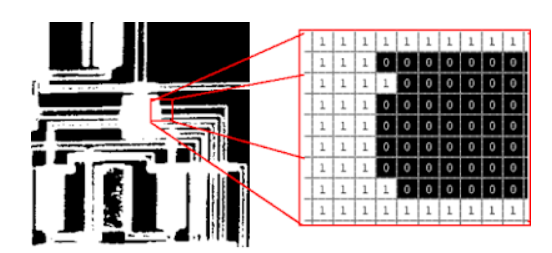
\includegraphics[width=\columnwidth]{Figures/insect2/binarynumber}
	\caption{ภาพแบบ Binary}{ที่มา: https://nextsoftwares.wordpress.com/2014/05/22/%E0%B8%84%E0%B8%A7%E0%B8%B2%E0%B8%A1%E0%B8%A3%E0%B8%B9%E0%B9%89%E0%B9%80%E0%B8%9A%E0%B8%B7%E0%B9%89%E0%B8%AD%E0%B8%87%E0%B8%95%E0%B9%89%E0%B8%99%E0%B9%80%E0%B8%81%E0%B8%B5%E0%B9%88%E0%B8%A2%E0%B8%A7/}
		\label{Fig:ิbinaryImage} 
	\end{figure}
	
	
	\begin{itemize}
		\item{Grayscale Image เป็นรูปที่เก็บโดยใช้รูปแบบของอาร์เรย์ 2 มิติ โดยค่าที่เก็บจะมีค่าอยู่ในช่วงๆหนึ่ง ซึ่งระดับของสีขึ้นอยู่กับขนาดของบิตที่ใช้เก็บค่าสี ดังรูปที่ \ref{Fig:ิGrayscaleImage}
		}
	\end{itemize}
	
	\begin{figure}[H]
		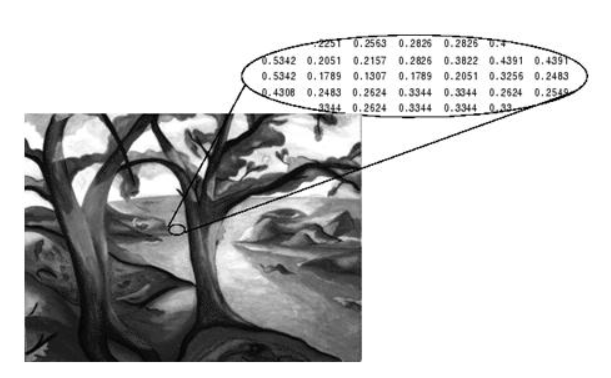
\includegraphics[width=\columnwidth]{Figures/insect2/GS}
		\caption{ภาพแบบ Grayscale Image}{ที่มา: https://nextsoftwares.wordpress.com/2014/05/22/%E0%B8%84%E0%B8%A7%E0%B8%B2%E0%B8%A1%E0%B8%A3%E0%B8%B9%E0%B9%89%E0%B9%80%E0%B8%9A%E0%B8%B7%E0%B9%89%E0%B8%AD%E0%B8%87%E0%B8%95%E0%B9%89%E0%B8%99%E0%B9%80%E0%B8%81%E0%B8%B5%E0%B9%88%E0%B8%A2%E0%B8%A7/}
			\label{Fig:ิGrayscaleImage} 
		\end{figure}
		
		\begin{itemize}
			\item{RGB Image หรือ Truecolor Image เป็นรูปที่เก็บโดยใช้อาร์เรย์ 3 มิติ ขนาด m x n x 3 โดยที่ m คือความยาว และ n คือความกว้างของภาพในหน่วยพิกเซล ส่วนมิติสุดท้ายนั้น ในแต่ละมิติจะเก็บค่าสีแยกกัน คือสีแดง (Red) สีเขียว (Green) และสีน้ำเงิน (Blue) ดังรูปที่ \ref{Fig:ิRGBImage}
			}
		\end{itemize}
		
		\begin{figure}[H]
			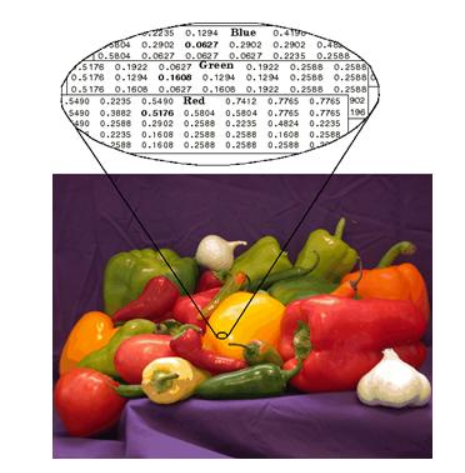
\includegraphics[width=\columnwidth]{Figures/insect2/RGB}
			\caption{ภาพแบบ RGB Image}{ที่มา: https://nextsoftwares.wordpress.com/2014/05/22/%E0%B8%84%E0%B8%A7%E0%B8%B2%E0%B8%A1%E0%B8%A3%E0%B8%B9%E0%B9%89%E0%B9%80%E0%B8%9A%E0%B8%B7%E0%B9%89%E0%B8%AD%E0%B8%87%E0%B8%95%E0%B9%89%E0%B8%99%E0%B9%80%E0%B8%81%E0%B8%B5%E0%B9%88%E0%B8%A2%E0%B8%A7/}
				\label{Fig:ิRGBImage} 
			\end{figure}
			\subsection{Machine Leaning}
			Machine Learning คือ ส่วนการเรียนรู้ของเครื่อง ถูกใช้งานเสมือนเป็นสมองของ AI (Artificial Intelligence) เราอาจพูดได้ว่า AI ใช้ Machine Learning ในการสร้างความฉลาด มักจะใช้เรียกโมเดลที่เกิดจากการเรียนรู้ของปัญญาประดิษฐ์ ไม่ได้เกิดจากการเขียนโดยใช้มนุษย์ มนุษย์มีหน้าที่เขียนโปรแกรมให้ AI 
			(เครื่อง) เรียนรู้จาก ข้อมูลเท่านั้น ที่เหลือเครื่องจัดการเอง Machine Learning เรียนรู้จากสิ่งที่เราส่งเข้าไปกระตุ้นแล้วจดจำเอาไว้เป็นมันสมอง ส่งผลลัพธ์ออกมาเป็นตัวเลข code หรือ ที่ส่งต่อไปแสดงผล หรือให้เจ้าตัว AI นำไปแสดงการกทำ Machine Learning เองสามารถเอาไปใช้งานได้หลายรูปแบบ ต้องอาศัยกลไกที่เป็นโปรแกรม หรือเรียกว่า Algorithm ที่มีหลากหลายแบบโดยมี Data Scientist เป็นผู้ออกแบบ หนึ่งใน Algorithm ที่ได้รับความนิยมสูง คือ DeepLearning ซึ่งถูกออกแบบมาให้ใช้งานได้ง่าย และประยุกต์ใช้ได้หลายลักษณะงาน อย่างไรก็ตาม ในการทำงานจริงของ Data Scientist จำเป็นต้องออกแบบตัวแปรต่างๆ ทั้งในตัวของ Deep Learning เองและต้องหา Algorithm อื่นๆ มาเป็นคู่เปรียบเทียบ เพื่อมองหา Algorithm ที่เหมาะสมที่สุดในการใช้งานจริง
			
			Algorithm ที่นำมาใช้ในการวิเคราะห์ ในส่วนของฟังก์ชันคือกฎความสัมพันธ์(Associations) การทำเหมืองข้อมูลเพื่อหาความสัมพันธ์ของเหมืองข้อมูลมักใช้ในธุรกิจการค้าปลีก(retailing Business) เช่น ร้านค้าสะดวกซื้อ หรือ ซุปเปอร์มาเก็ต เป็นการวิเคราะห์การตลาด(Marketing basket Analysis) เพื่อศึกษาพฤติกรรมการซื้อสินค้าของลูกค้า และหาความสัมพันธ์ของสินค้าที่ลูกค้าซื้อ
			
			ความสัมพันธ์ของสินค้าที่ลูกค้าซื้อจะแสดงในรูปของกฎความสัมพันธ์  Association Rule ดังนี้
			
			\begin{figure}[H]
				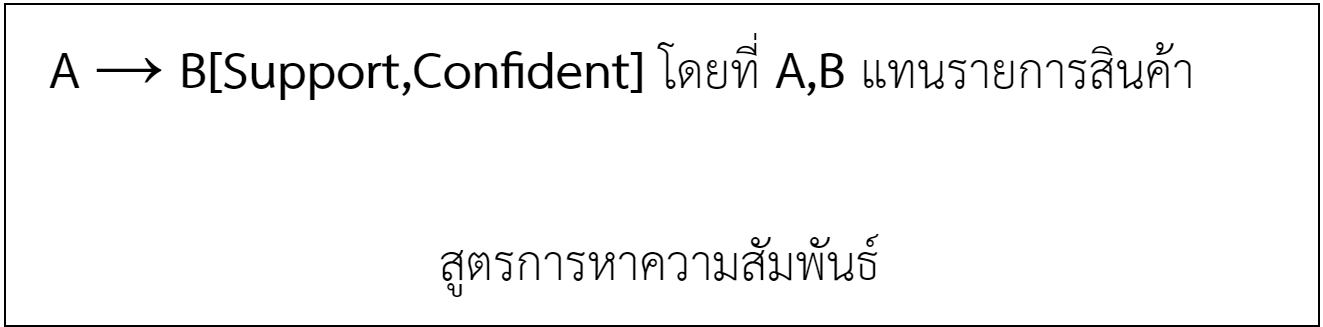
\includegraphics[width=\columnwidth]{Figures/insect2/AS}
				\caption{สูตรการหาความสัมพันธ์ Association Rule}
				\label{Fig:AS} 
			\end{figure}
		
			 
			 \newline
			 เช่น Milk -> Eggs [Support = 25 เปอร์เซ็น ,Confident=33.34 เปอร์เซ็น] หมายความว่า 25เปอร์เซ็น ของทรานแซคชั่นทั้งหมด ลูกค้า จะซื้อนม (Milk) และซื้อไข่ (Eggs) พร้อมกันและ 33.34 เปอร์เซ็น ของลูกค้าที่ซื้อนมแล้วจะซื้อไข่ด้วย กฎความสัมพันธ์ที่สนใจหรือกฎความสัมพันธ์ที่แข็งแกร่ง (Strong Association Rules) คือ กฎความสัมพันธ์ที่มีค่าสนับสนุน (support) และค่าความเชื่อมั่น (confidence) ผ่านเกณฑ์ขั้นต่ำ(Minimum Threshold) ที่ผู้วิเคราะห์ข้อกำหนดขึ้นมา
			  
			  
	     	\end{figure}
			\section{ความรู้พื้นฐานเกี่ยวกับ Pillow}
			Pillow  เป็น  Library ด้านความสามารถในการประมวลผลภาพและกราฟฟิก หรือโมดูลจัดการและประมวลผลรูปภาพบน Python ใน Python มีโมดูลด้านที่ชื่อว่า Python Imaging Library (PIL) ซึ่งรองรับแต่ Python 2  จึงมีคนมาพัฒนาเป็นโมดูล Pillow  ที่รองรับทั้ง Python 2 และ Python 3  โมดูล Pillow สามารถจักการจัดเก็บรูปภาพ (Image Archives) แสดงรูปภาพ (Image Display) ประมวลผลรูปภาพ เช่น ปรับขนาดรูปภาพ แปลงไฟล์รูปภาพ ใส่ตัวอักษรลงในภาพ และอื่น ๆ เป็นต้น ดังรูปที่ \ref{Fig:pillow}
			
			\begin{figure}[H]
				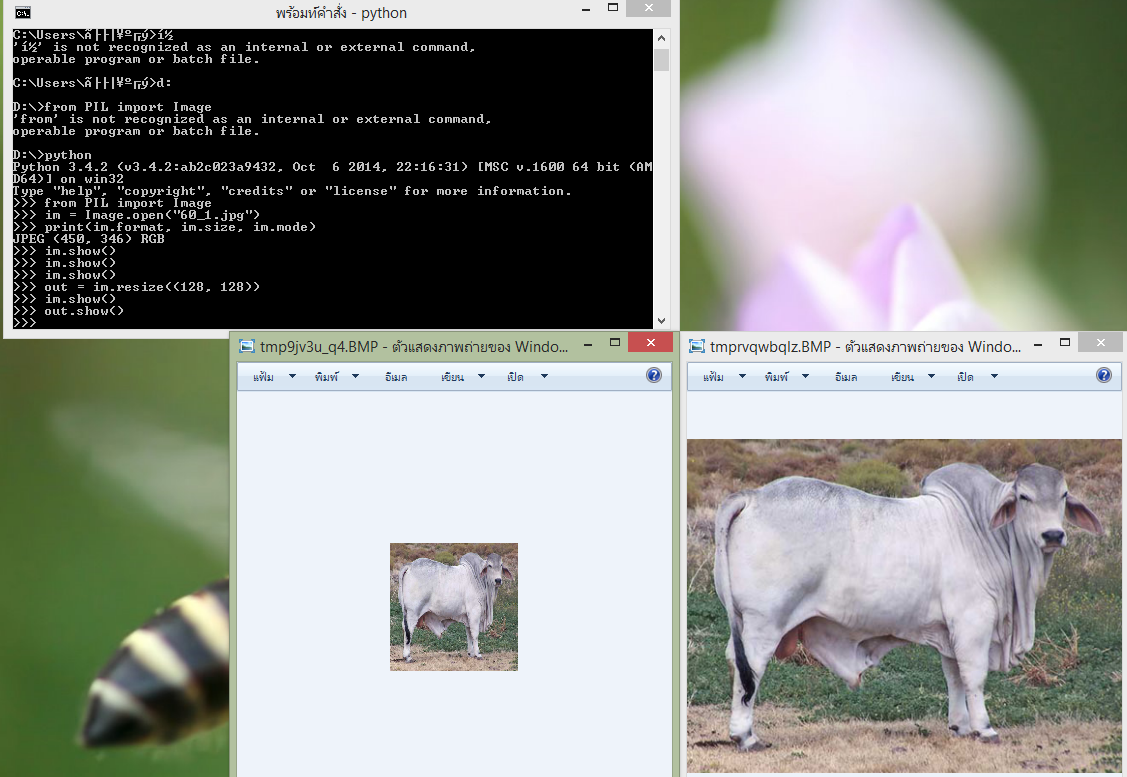
\includegraphics[width=\columnwidth]{Figures/insect2/pillow}
				\caption{การขยายรูปโดยใช้ Pillow}{ที่มา: https://python3.wannaphong.com/2014/11/image-processing-python.html}
				\label{Fig:pillow} 
			\end{figure}
		\section{MySQL}
		MySQL  คือ โปรแกรมระบบจัดการฐานข้อมูล ที่พัฒนาโดยบริษัท MySQL AB มีหน้าที่เก็บข้อมูลอย่างเป็นระบบ รองรับคำสั่ง SQL เป็นเครื่องมือสำหรับเก็บข้อมูลที่ต้องใช้ร่วมกับเครื่องมือหรือโปรแกรมอื่นอย่างผสมผสาน เพื่อให้ได้ระบบงานที่รองรับความต้องการของผู้ใช้ เช่น ทำงานร่วมกับเครื่องบริการเว็บ (Web Server) เพื่อให้บริการแก่ภาษาสคริปต์ที่ทำงานฝั่งเครื่องบริการ Server-Side Script เช่น ภาษา PHP ภาษา ASP.NET หรือภาษา JSP เป็นต้น หรือทำงานร่วมกับโปรแกรมประยุกต์ (Application Program) เช่น ภาษาวิชวลเบสิกดอทเน็ต (Visual Basic.NET) ภาษาจาวา (JAVA) หรือภาษาซีชาร์ป (C\#) เป็นต้น โปรแกรมถูกออกแบบให้สามารถทำงานได้บนระบบปฏิบัติการที่หลากหลาย และเป็นระบบฐานข้อมูลโอเพนซอร์ส (Open Source) ที่ถูกนำไปใช้งานมากที่สุด
		
		ความสามารถและการทำงานของโปรแกรม MySQL มีดังต่อไปนี้ 
		
		\begin{itemize}
			\item{MySQL (DataBase Management System : DBMS) 
				เป็นฐานข้อมูลที่มีลักษณะเป็นโครงสร้างของการเก็บรวบรวมข้อมูล การที่จะเพิ่ม เข้าถึงหรือประมวลผลข้อมูลที่เก็บในฐานข้อมูลจำเป็นจะต้องอาศัยระบบจัดการฐานข้อมูล ซึ่งจะทำหน้าที่เป็นตัวกลางในการจัดการกับข้อมูลในฐานข้อมูลทั้งสำหรับการใช้งานเฉพาะ และรองรับการทำงานของแอปพลิเคชันอื่นๆ ที่ต้องการใช้งานข้อมูลในฐานข้อมูล เพื่อให้ได้รับความสะดวกในการจัดการกับข้อมูลจำนวนมาก MySQL ทำหน้าที่เป็นทั้งตัวฐานข้อมูลและระบบจัดการฐานข้อมูล}
			\item{MySQL เป็นระบบจัดการฐานข้อมูลแบบ relational 
				ซึ่งฐานข้อมูลแบบ relational จะทำการเก็บข้อมูลทั้งหมดในรูปแบบของตารางแทนการเก็บข้อมูลทั้งหมดลงในไฟล์ เพียงไฟล์เดียว ทำให้ทำงานได้รวดเร็วและมีความยืดหยุ่น นอกจากนั้น แต่ละตารางที่เก็บข้อมูลสามารถเชื่อมโยงเข้าหากันทำให้สามารถรวมหรือจัดกลุ่มข้อมูลได้ตามต้องการ โดยอาศัยภาษา SQL ที่เป็นส่วนหนึ่งของโปรแกรม MySQL ซึ่งเป็นภาษามาตรฐานในการเข้าถึงฐานข้อมูล}
			\item{MySQL แจกจ่ายให้ใช้งานแบบ Open Source คือ ผู้ใช้งาน MySQL ทุกคนสามารถใช้งานและปรับแต่งการทำงานได้ตามต้องการ สามารถดาวน์โหลดโปรแกรม MySQL ได้จากอินเทอร์เน็ต (Internet) และนำมาใช้งานโดยไม่มีค่าใช้จ่าย}
		\end{itemize}
		
		\section{XAMPP}
		การพัฒนาเว็บไซต์ หรือโปรแกรมที่ทำงานบนเว็บแอปพลิเคชัน จำเป็นต้องอาศัยเครื่องแม่ข่ายเว็บ (Web server) ซึ่งอาจจะเป็นภาระสำหรับผู้เรียน หรือผู้พัฒนาบางกลุ่ม แนวทางหนึ่งที่นิยมกันคือ การจำลองเครื่องพีซีให้เป็นเครื่องแม่ข่ายเว็บด้วยโปรแกรมสำเร็จรูป ซึ่งมีให้เลือกหลายค่ายซึ่ง
		XAMPP เป็นหนึ่งในผลิตภัณฑ์ที่มีการพัฒนาออกมาให้ใช้งาน
		
		XAMPP  พัฒนาโดยโครงการ Apache Friends ที่เป็นโครงการไม่แสวงหาผลกำไร ที่จัดตั้งในปี ค.ศ. 2002 โดย Kai ‘Oswald’ Seidler และ Kay Vogelgesang ทั้งนี้ XAMPP ประกอบด้วยโปรแกรมย่อยได้แก่ โปรแกรม Apache โปรแกรมฐานข้อมูล MySQL โปรแกรมภาษา PHP และภาษา Perl อีกทั้ง XAMPP มีการปรับปรุงรุ่นอย่างต่อเนื่องเพื่อให้ทำงานได้กับระบบปฏิบัติการทั้ง Microsoft Windows, Mac OS x, Linux และ Solaris นอกจากนี้ยังไม่มีค่าใช้จ่ายในการดาวน์โหลดใช้งาน
		
		แนวคิดของ XAMPP
		
		XAMPP โปรแกรมรวมการติดตั้งสำหรับนักพัฒนาโปรแกรมของ Apache เพื่อที่ให้โปรแกรมนั้นใช้งานง่ายและสะดวกสำหรับนักพัฒนาโปรแกรม โปรแกรม XAMPP นั้นได้ตั้งค่าเริ่มต้น ให้สามารถใช้งานโปรแกรม XAMPP แบบใช้งานโปรแกรมได้ในทุกอย่าง (all features turn on)
		ค่ามาตรฐานนี้ อาจจะเป็นจุดอ่อนในเรื่องความปลอดภัย หากนำไปใช้ในเครื่องที่ใช้งานจริง เพราะโปรแกรม XAMPP ถูกออกแบบมาสำหรับเครื่องของนักพัฒนาโปรแกรม
		
		ประโยชน์ของ XAMPP
		\begin{itemize}
			\item สะดวกในการติดตั้งและถอนการติดตั้ง
			\item โปรแกรมมีคำสั่งต่างๆ ทำให้ง่ายต่อการใช้งาน
			\item โปรแกรมสามารถใช้งานได้ในหลายระบบปฏิบัติการ เช่น  Linux, Windows, Mac OSX หรือ ระบบปฏิบัติการอื่นๆ
			\item เป็นโปรแกรมฟรีที่สนับสนุนในการใช้งานของผู้ที่ต้องการพัฒนาระบบ 
		\end{itemize}
		
			
			\section{ความรู้พื้นฐานเกี่ยวกับปัญญาประดิษฐ์ (Artificial Intelligence)}
			ปัญญาประดิษฐ์ (AI) เป็นศาสตร์แขนงหนึ่งของวิทยาศาสตร์ คอมพิวเตอร์ ที่เกี่ยวข้องกับวิธีการทำให้คอมพิวเตอร์มีความสามารถคล้ายมนุษย์ หรือเลียนแบบพฤติกรรมมนุษย์ โดยเฉพาะความสามารถในการคิดเองได้ หรือมีปัญญานั่นเอง ปัญญานี้มนุษย์เป็นผู้สร้างให้คอมพิวเตอร์ จึงเรียกว่าปัญญาประดิษฐ์  
			
			\subsection{โครงข่ายประสาทเทียม (Neural Network) }
			โครงข่ายประสาทเทียม  คือ โครงข่ายประสาทเทียมที่เป็นการจำลองมาจากสมองของมนุษย์ เพื่อจำลองการทำงานของเครือข่ายประสาทในสมองมนุษย์ ด้วยวัตถุประสงค์ที่จะสร้างเครื่องมือ ซึ่งมีความสามารถในการเรียนรู้การจดจำรูปแบบ (Pattern Recognition) และการสร้างความรู้ใหม่ (Knowledge Extraction) เช่นเดียวกับความสามารถที่มีในสมองมนุษย์นั่นเอง
			หลักการของ Neural Network 
			ในคอมพิวเตอร์ neurons ประกอบด้วย input และ output เหมือนกัน โดยจำลองให้ input แต่ละอันมี weight เป็นตัวกำหนดน้ำหนักของ input โดย neuron แต่ละหน่วยจะมีค่า threshold เป็นตัวกำหนดว่าน้ำหนักรวมของ input ต้องมากขนาดไหนจึงจะสามารถส่ง output ไปยัง neurons ตัวอื่นได้ เมื่อนำ neuron แต่ละหน่วยมาต่อกันให้ทำงานร่วมกันการทำงานนี้ในทางตรรกแล้ว จะเหมือนกับปฏิกิริยาเคมีที่เกิดในสมอง เพียงแต่ในคอมพิวเตอร์ทุกอย่างเป็นตัวเลขเท่านั้นเอง ดังรูปที่ \ref{Fig:CNN}
			\begin{figure}[H]
				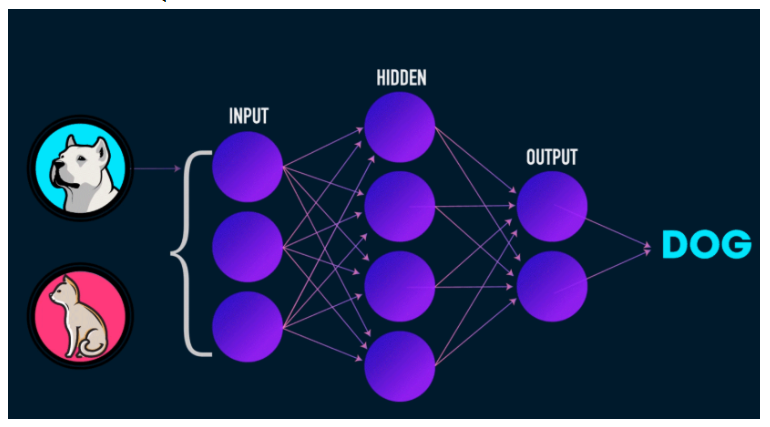
\includegraphics[width=\columnwidth]{Figures/insect2/NN}
				\caption{ขั้นตอนของโครงข่ายประสาทเทียมแบบคอนโวลูชันนัล}{ที่มา: https://analyticsindiamag.com/most-common-activation-functions-in-neural-networks-and-rationale-behind-it/}
				\label{Fig:CNN} 
			\end{figure}

          \section{งานวิจัยที่เกี่ยวข้อง}
          นางสาวสุภาภรณ์ จินดาวงษ์ ได้นำเสนอวิจัยเกี่ยวกับ การศึกษาพฤติกรรมการเลอืกใช้บริการร้านกาแฟสดของผู้บริโภค ผู้ศึกษาจึงสนใจเกี่ยวกับ พฤติกรรมการเลือกใช้บริการร้านกาแฟสดของผู้บริ โภคในอำเภอเมือง จังหวัด นครปฐม กรณีศึกษา ร้านบ้านไร่กาแฟ สาขาที่29 เพื่อทราบถึงเหตุผลการเข้าใช้บริการร้านกาแฟสดบ้านไร่กาแฟ สาขาที่29 ผลการวิจัยทำให้
          สามารถใช้เป็นแนวทางในการปรับปรุงธุรกิจให้ตรงกับความตอ้งการผู้บริโภคและเป็นแนวทาง
          ดำเนินกิจการแก่ผู้สนใจธุรกิจร้านกาแฟ
		  
		  	
		  นางสาวกานดา เสือจำศิล ได้นำเสนอวิจัยเกี่ยวกับ พฤติกรรมการเข้าใช้บริการร้านกาแฟสด อเมซอน ของผู้บริโค เพื่อศึกษาพฤติกรรมการเข้าใช้บริการร้านกาแฟสด อเมซอน ปัจจัยส่วนบุคคลของผู้บริโภคที่เข้าใช้บริการร้านกาแฟสด อเมซอน และปัจจัยส่วนผสมทางการตลาดต่อการเข้าใช้บริการร้านกาแฟสด อเมซอน กลุ่มตัวอย่างที่ใช้ คือ ผู้บริโภคในจังหวัดปทุมธานีที่เข้าใช้บริการร้านกาแฟสด อเมซอน จำนวน 400 คน
		  \newline
		  	

	
